\section{Construction des perturbations}
%     \begin{verbatim}
% - on s'intéresse aux perturbations de type replace pour travailler sur l'impact des mots importants
% (car liés au vocabulaire de spécialité) en les replaçant
% - La conception de perturbations necessite de bien choisir les mots à remplacer (traité dans la sous partie 1) et les mots remplaçants (traité dans la sous partie 2). 
% - La sous partie 3 propose un nouveau type de perturbations
%     \end{verbatim}

    Dans un premier temps, on se concentre sur les perturbations de type \replace. Cela permet d'exploiter la multiplicité des sens (polysémie) de certains mots de spécialité en jouant sur leur sens de spécialité et leur sens commun ou issu d'une autre spécialité. \\
    Pour construire des perturbations de type \replace qui impactent le modèle et qui soient pertinentes à interpréter, il faut bien choisir le mot à remplacer et le mot remplaçant. On propose aussi un nouveau type de perturbation.

    \subsection{Identification des mots cibles}
%         \begin{verbatim}
% - Le choix des remplaçant est fait par jugement humain
% - Le choix des mots à remplacer se fait à l'aide de 
%     - fréquence dans l'échantillon de données sélectionné
%     - IDF 
%     - appartenance au vocabulaire de spécialité (jugement humain)
%     - présence du mot dans la question étudiée (cas du dataset à 1! question)
% - la bonne couverture des documents est importante (commentaire sur NaN) 
% pour avoir des résultats lisibles
% - cas du voc de spécialité : ne pas être un stop word / les critères précédents permettent en association avec un doci ou un simple jugement humain d'identifier le vocabulaire de spécialité
%         \end{verbatim}


        Pour qu'une perturbation de type \replace impacte de façon pertinente le modèle, elle doit remplacer des mots bien choisis.
        On propose les critères suivants pour sélectionner des mots cibles pour impacter le modèle :
        \begin{itemize}
            \item Fréquence du mot dans le dataset
            \item L'IDF du mot dans le dataset
            \item La présence du mot dans la question ciblée
        \end{itemize}

        
        Les indicateurs de fréquence permettent de faciliter l'identification du vocabulaire de spécialité. On peut aussi s'aider d'un dictionnaire. Un intérêt particulier doit être porté aux mots ayant un sens spécifique ou différent dans le contexte de la spécialité visée. Ces mots permettent d'exploiter la polysémie lors de la construction de perturbations.

        \begin{table}[!ht]
            \centering
            \begin{tabular}{|l|l|l|}
            \hline
                Mot & Fréquence & TF-IDF \\ \hline \hline
                \textbf{matériel} & 16 & 0.063 \\ \hline
                \textbf{système} & 11 & 0.054 \\ \hline
                \textbf{limitation} & 6 & 0.050 \\ \hline
                \textbf{drone} & 10 & 0.044 \\ \hline
                \textbf{défense} & 10 & 0.044 \\ \hline
                prendre & 6 & 0.043 \\ \hline
                compte & 5 & 0.040 \\ \hline
                action & 8 & 0.040 \\ \hline
                \textbf{article} & 9 & 0.040 \\ \hline
                ministre & 8 & 0.039 \\ \hline
                \textbf{aérien} & 7 & 0.037 \\ \hline
                acteur & 6 & 0.034 \\ \hline
                guerre & 8 & 0.034 \\ \hline
                informationnel & 5 & 0.031 \\ \hline
                information & 6 & 0.030 \\ \hline
            \end{tabular}
            \caption{Mots importants du troisième dataset d'exemple}
            \label{tab:StatsDatasetV3}
        \end{table}

        La table~\ref{tab:StatsDatasetV3} présente, après lemmatisation des documents, les statistiques du vocabulaire présent pour les 15 plus grands TF-IDF. Tous les mots ayant un fort TF-IDF ne sont pas intéressant à remplacer. On se concentre sur les mot appartenant au vocabulaire de la défense et disposant d'au moins un autre sens. On inclus aussi les mots porteurs de sens ou d'information de la question du dataset. En les modifiants, on s'attend à une fort impact sur la pertinence du document. On choisi de se concentrer sur les mots indiqués en gras ainsi que sur le mot \textit{technique} car il est porteur de sens dans le question.


    \subsection{Perturbations de type \replace basées sur les synonymes}
%         \begin{verbatim}
% - On propose plusieurs candidats au remplacement classé en 4 niveaux ...
% - Rq : il faudrait fonder l'estimation du niveau des perturbations

% niveau 1 : Observer la distinction entre sens et le mot lui-même (on ne s'attend pas à un effet fort
% sauf en cas d'erreur sur le sens du mot remplacé)
% Niveau 2 : Forcer l'erreur d'interprétation du mot en exploitant le polysémie 
% Niveau 3 : Remplacement absurde. Il ne laisse pas d'indice sur le mot supposé être présent
% Niveau 4 : Est une expression absurde mais grammaticalement correcte et non liée au mot remplacé
%         \end{verbatim}

        Une fois le mot à remplacer choisi, on propose dans un premier temps d'exploiter la polysémie (les multiples sens) de ce mot. On distingue deux groupes de candidats : les synonymes (ou mot proche) du mot remplacé partageant le sens du vocabulaire de spécialité et les synonymes (ou mot proche) du mot remplacé ayant un autre sens. Ces groupes de mots remplaçants reflètent deux niveaux de perturbation. Les perturbations de niveau 1 remplacent le mot par un synonyme du mot remplacé ayant le sens du vocabulaire de spécialité ciblé. Par exemple, dans le domaine du droit, remplacer défense par interdiction est une perturbation de niveau 1. Les perturbations de niveau 2 remplacent le mot ciblé par un mot proche mais dans un autre sens que le domaine de spécialité visé. Dans l'exemple précédent, remplacer défense par corne est une perturbation de niveau 2. 

        Les seconde et troisième colonnes de la table~\ref{tab:perturbations} présentent les mots remplaçants retenus pour les mots ciblés choisis dans l'exemple de la sous-section précédente. Dans le contexte de la défense, \textit{aérien} qualifie des véhicules ou objets se déplaçant en volant. L'expression \textit{de vol} est un bon candidat pour construire une perturbation de niveau 1. Sur le même principe, le secteur de la défense vise à protéger un territoire et/ou une population.  Remplacer \textit{défense} par \textit{protection} est une perturbation de niveau 1.  À contrario, qualifier un mouvement ou une démarche d'aérien ou de poétique ne correspond pas à l'usage fait dans la défense. \textit{poétique} est un mot remplaçant adapté pour une perturbation de niveau 2. De même, la défense d'un éléphant peut être comparée à une corne de rhinocéros mais le sens donné à \textit{défense} dans ce contexte n'est pas le même. Remplacer \textit{défense} par \textit{corne} est une perturbation de niveau 2. Les distributions des scores de pertinence des documents pour ces quatre perturbations sont disponibles dans la figure~\ref{fig:pertNiv1-2}.

        \begin{figure}
            \centering
            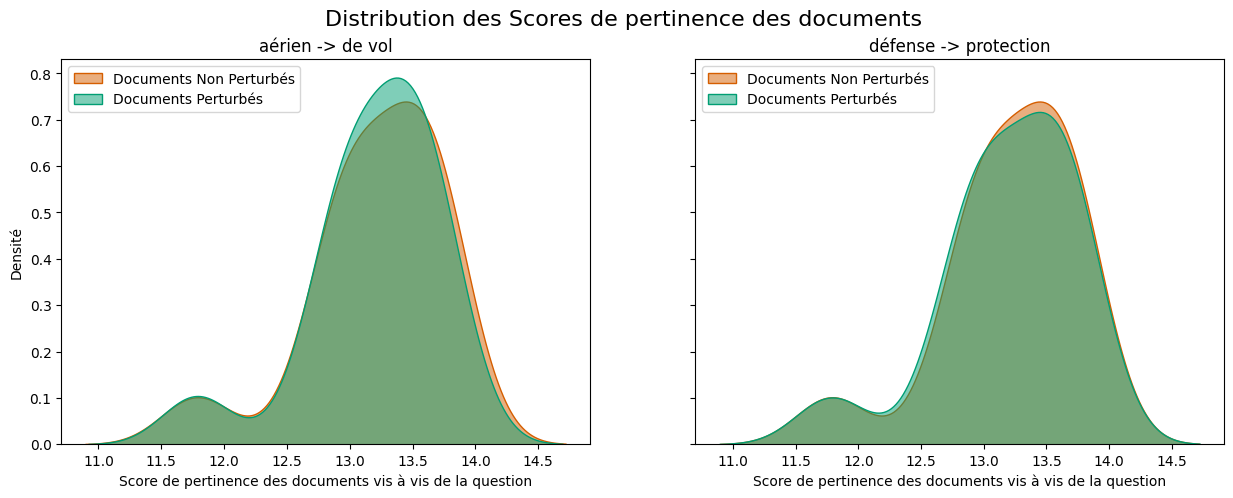
\includegraphics[width=0.8\linewidth]{images/PerturbationScoreExemple_Synonyme.png}\\
            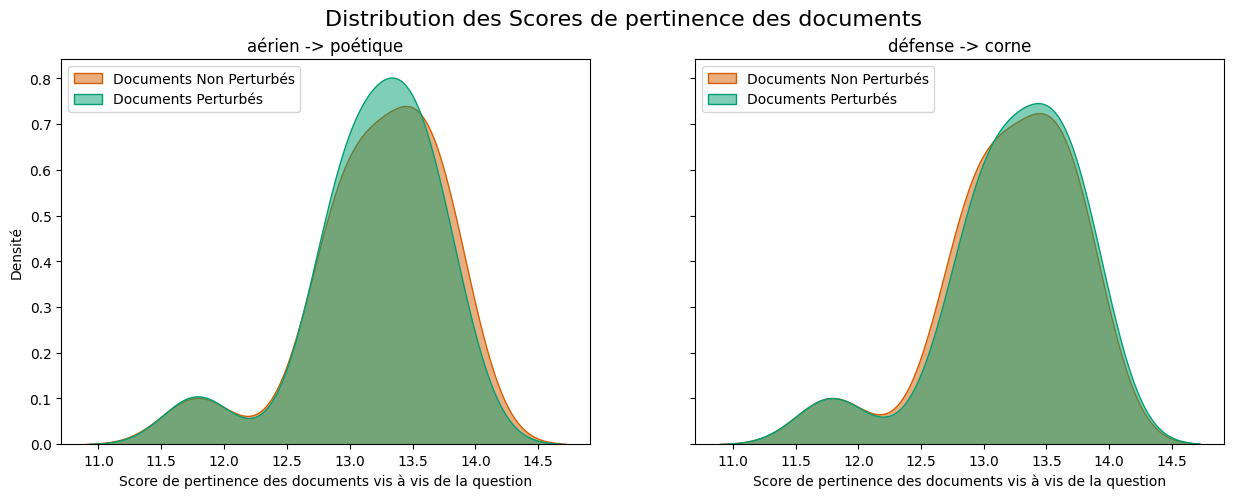
\includegraphics[width=0.8\linewidth]{images/PerturbationScoreExemple_Polysemie.png}
            \caption{Distribution des scores de pertinence pour les exemples de perturbation de niveau 1 et 2}
            \label{fig:pertNiv1-2}
        \end{figure}

        Les perturbations de niveau 1 et 2 listés dans la table~\ref{tab:perturbations} n'impactent pas suffisamment le modèle. Cela nous a surpris car les résultats présentés par \cite{parry_mechir_2025} exploitaient aussi la polysémie et donnaient des perturbations plus impactantes. En prenant un peu de recul, les grand modèles de langue semblent pouvoir manipuler différents sens pour un mot. Cela était moins le cas pour les modèles peu profonds tels que Word2Vec qui tendent à regrouper tous les sens ou les écraser au profit du plus présent. Il est possible que les perturbations exploitant la polysémie (perturbations de niveau 2) laissent suffisamment d'indices pour que les grand modèles gèrent cette difficulté. Cela pourrai expliquer le faible impact des perturbations de niveau 2 sur mE5.

        %Les perturbations de niveau 1 et 2 n'ont pas nécessairement un impact suffisant sur le modèle. Les grand modèles de langue basés sur l'apprentissage profond sont réputés pour gérer les difficultés liées à la polysémie des mots. 
        %\md{Pourquoi on a dit ça en réunion il y a 3 mois? Je n'ai aucune idée de référence pour attester de ça.}
        %Il n'est donc pas si étonnant que les perturbations de niveau 1 ou 2 n'impactent que peu mE5.
        %\alh{plus précisément nous avions dit que les embedding contextuels permettaient de mieux sélectionner le sens d'un mot en contexte dans le cas de la polysémie, par exemples les embeddings non profonds type word2vec n'ont qu'une seule entrée pour avocat et tous les sens sont mergés, tandis que Bert gère parfaitement la polysémie. A partir de là, on s'est dit que mE5 était tolérant à l'inexactitude si dans le cadre de la polysémie il y avait une relation sémantique. Par exemple corne pour défense, on suppose qu'une relation sémantique même lointaine laisse le système une possibilité de gérer mais il est vrai qu'à ben y réfléchir ce n'est pas si évident. on avait bon espoir au départ que cela impacte plus puisqu'on tranchait avec le sens initial mais on a été déçue : ), probablement parce que l'éloignement dans l'espace sémantique n'est pas si grand...? En vrai on n'en sait rien.}

        \subsection{Perturbations de type \replace plus agressives}
        
        On propose deux niveaux de perturbation supplémentaires effectuant des replacements plus prononcés. Les perturbations de niveau 3 remplacent le mot ciblé par un mot n'ayant aucun lien avec les différents sens du mot ciblé. 
%         \color{teal}
%         Ici 2 sources : Ce que le CNRTL nomme \href{https://www.cnrtl.fr/lexicographie/incompatibilit%C3%A9}{"incompatibilité"}
%         suivant \cite{greimas_semiotique_1979} est :
%         \begin{quote}
%             "Impossibilité, pour deux éléments sémiotiques quelconques, de contracter une relation".
%         \end{quote}
        
%         \cite{majewska_semantic_2021} quant à eux ont cherché à faire construire physiquement une esapece sémantique par des humains. Il arrivent à une expression de faible "\textit{relatedness}" qui reprend grossièrement l'idée d'incompatibilité exprimée plus haut. Donc on a 1. synonyme, 2. synonyme d'un autre sens dans la polysémie 3. terme "incompatible" "unrelated" 4. combinaison de 2 termes incompatibles entre eux et incompatible avec la cible. Une chose qui pourrait marcher pour asseoir cette méthodo c'est de calculer la distance avec un Word2Vec tout bête, une fois entrainé sur votre corpus :
%         mon code pour calculer cela sur un autre corpus juste après(rien d'interessant, juste que pour le faire tourner j'ai tout ramener à des des mminuscules, sans stopword, etc. puis j'ai créer le model, puis utiliser wv.similarity, si j'avais eu le copru sje l'aurais fait vite fait). Sinon on pourrait aussi calculer le plus court chemin entre source et cible dans des ressource du type JeuxdeMots (\href{https://www.jeuxdemots.org/jdm-about.php}{https://www.jeuxdemots.org/jdm-about.php}, mais le dump est très lourd, c'est casse pied à faire.
% \begin{verbatim}
% import pandas as pd
% from gensim.models import Word2Vec

% df = pd.read_csv("https://www.data.gouv.fr/api/1/datasets/r/3a6d6fe3-8548-43ed-ad09-72052771447c")
% df["avis_word_token"] = df["Avis"].map(lambda x : word_tokenize(x.replace("'", " "))) 
% df["avis_word_token"] = df["avis_word_token"].map(lambda list_word: [word.lower()  for word in list_word if word.isalpha()])
% custom_stopwords = ["a", "dont", "madame", "monsieur", "peut", "dès", "lors", "être", "ce",
%                     "ces", "cet", "cette", "comme", "ainsi", "si"]
% stopwords_fr = stopwords.words('french') + custom_stopwords
% df["avis_word_token"] = df["avis_word_token"].map(lambda list_word: [word for word in list_word if word not in stopwords_fr])
% sentences = df["avis_word_token"].tolist()
% model = Word2Vec(sentences, window=5, min_count=5, workers=4)
% model.wv.similarity("défense","corne")
% \end{verbatim}
%         \color{black}
        On conserve juste la même nature entre le mot remplacé et le mot remplaçant (les noms sont remplacés par des noms, les adjectifs par des adjectifs,...). Ces perturbations ne donnent aucune piste sur le mot initialement présent ce qui rend la compréhension plus difficile. Les perturbations de niveau 4 sont encore plus agressives. Le mot est remplacé par un groupe de mot absurde (ex: luge pontificale). Ces perturbations masquent les mots cibles qui sont identifiés comme important par une groupe de mot qui n'est que du bruit. 

        Les quatrième et cinquième colonnes de la table~\ref{tab:perturbations}, donnent les perturbations de niveau 3 et 4 retenues pour les mots à remplacer choisis. Les mots remplaçants choisi pour les perturbation de niveau 3 restent de même nature (\textit{épicurien} est un adjectif comme \textit{aérien},...) mais sont sémantiquement éloignés du mot remplacé. Les groupes nominaux remplaçant pour les perturbations de niveau 4 sont bien des concepts qui ne sont pas réels. Les distributions des pertinences sont visualisés dans la figure~\ref{fig:pertNiv3-4}. On remarque d'ailleurs que les perturbations choisies n'impactent pas toujours le modèle autant qu'attendu.

        \begin{figure}
            \centering
            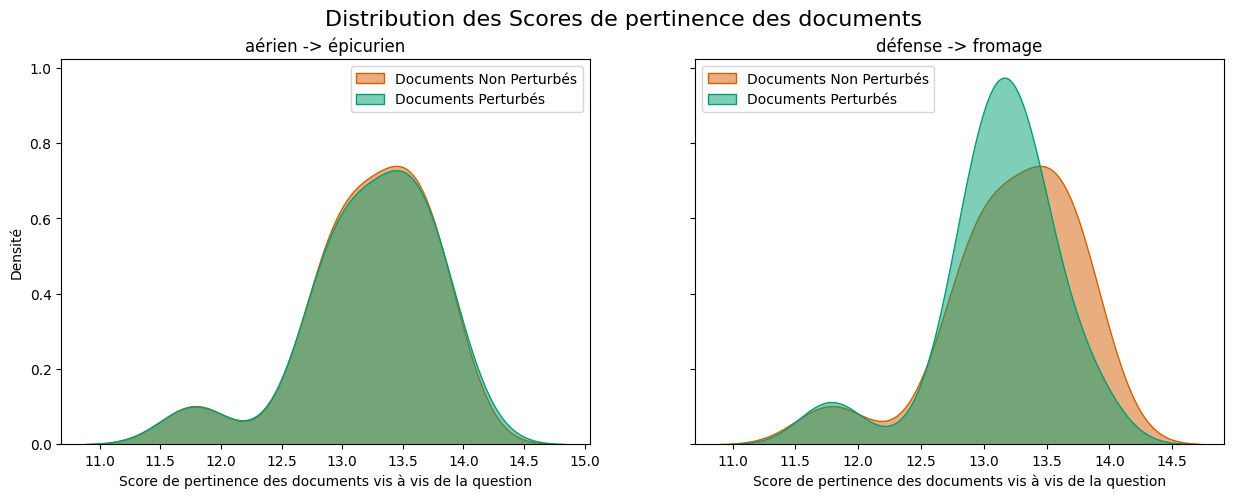
\includegraphics[width=0.8\linewidth]{images/PerturbationScoreExemple_Elephants.png}\\
            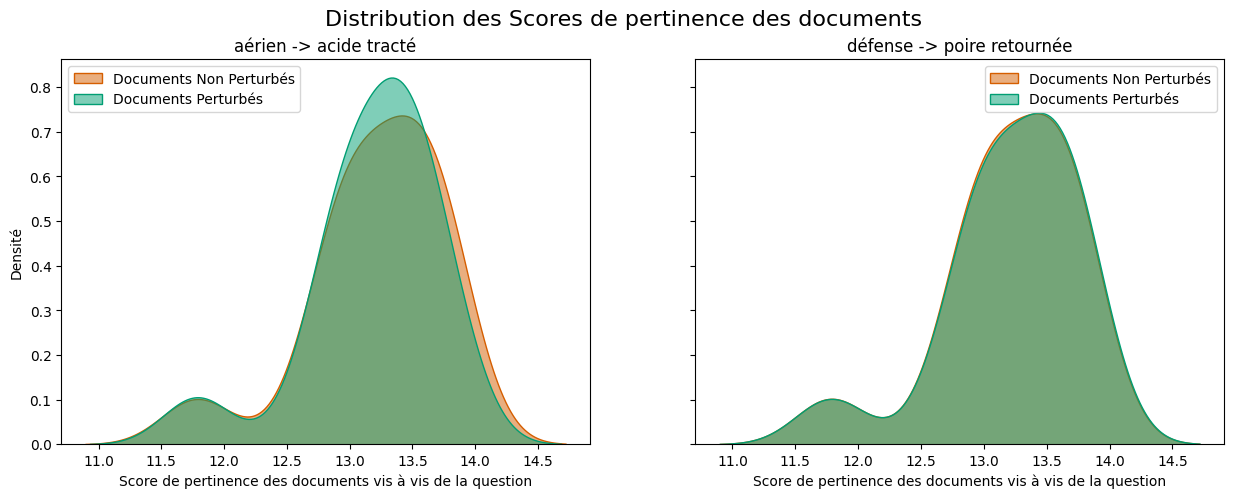
\includegraphics[width=0.8\linewidth]{images/PerturbationScoreExemple_ElephantsRoses.png}
            \caption{Distribution des scores de pertinence pour les exemples de perturbation de niveau 3 et 4}
            \label{fig:pertNiv3-4}
        \end{figure}

        La table~\ref{tab:niveauxPerturbation} récapitule les 4 niveaux de perturbation et les phénomènes observés.

        \begin{table}
            \centering

            \begin{tabular}{|c|p{0.3\linewidth}|p{0.3\linewidth}|p{0.3\linewidth}|}
                \hline
                 Niveau & Caractéristiques du mot remplaçant & Résultat attendu  & Caractéristique de nœud ou composant visé dans le modèle \\
                 \hline 
                 \hline
                 1 & synonyme (ou mot proche) ayant le sens du vocabulaire de spécialité visé & Faible perturbation &  Détection et prise en compte du mot ciblé spécifiquement \\
                 \hline
                 2 & synonyme (ou mot proche) ayant un sens différent de celui lié au vocabulaire de spécialité visé & Perturbation marquée. Quelques nœuds sensibles lors de l'application de l'activation patching & Détection et prise en compte du sens du vocabulaire de spécialité \\
                 \hline
                 3 & mot sans lien avec aucun sens du mot cible & Perturbation marquée. Quelques nœuds sensibles lors de l'application de l'activation patching & Prise en compte du sens de spécialité du mot ciblé. \\
                 \hline
                 4 & groupe de mot absurde sans lien avec la mot cible & Perturbation très marquée. Quelques nœuds sensibles lors de l'application de l'activation patching & Prise en compte du sens de spécialité du mot ciblé. \\
                 \hline
            \end{tabular}
            
            \caption{Récapitulatif des niveaux de perturbation proposé}
            \label{tab:niveauxPerturbation}
        \end{table}

        
        \begin{table}
            \centering
            \begin{tabular}{|l||l|l|l|l|}
            \hline
                Mot remplacé & Niveau 1 & Niveau 2 & Niveau 3 & Niveau 4 \\ \hline \hline
                aérien & de vol & poétique & épicurien & acide tracté \\ \hline
                article & sujet & déterminant & table & luge pontificale \\ \hline
                défense & protection & corne & fromage & poire retournée \\ \hline
                drone & vecteur & bourdon & gazon & ver de verre \\ \hline
                limitation & contrainte & bornage & animation & plastique anarchique \\ \hline
                matériel & outil & concret & post-it & porte sans poivre \\ \hline
                système & dispositif & ensemble & panneau & esperluette en vent \\ \hline
                technique & spécialisé & difficile & magique & feuille entubée \\ \hline
            \end{tabular}
            \caption{Perturbations proposées pour les mots à remplacer sélectionnés pour chaque niveau évoqué}
            \label{tab:perturbations}
        \end{table}

    \subsection{Perturbations de type \fullreplace}
%         \begin{verbatim}
% - pour augmenter le nombre de document perturbé et limiter l'impact d'un mot seulement dans la 
% cartographie (avoir un aperçu plus global), on propose un nouveau type de perturbation : full_replace
% - on étend les niveaux à ce nouveau type de perturbations
%         \end{verbatim}

        Une autre piste explorée pour augmenter l'impact des perturbations basées sur les synonymes est de cumuler plusieurs remplacements en même temps. On propose le nouveau type de perturbation \fullreplace qui applique une liste de perturbations de type \replace en une fois sur le document en guise de perturbation.  On étend les quatre niveaux de perturbation aux perturbations de type \fullreplace en considérant le niveau des perturbations \replace qu'elle inclus. \\
        Au delà de l'augmentation de l'impact de la perturbation sur le modèle, les perturbation \fullreplace permettent de s'affranchir du bruit introduit par chaque mot individuellement et de se concentrer sur un ensemble de composants du modèle sensible au vocabulaire de spécialité de façon plus globale.

        \begin{figure}
            \centering
            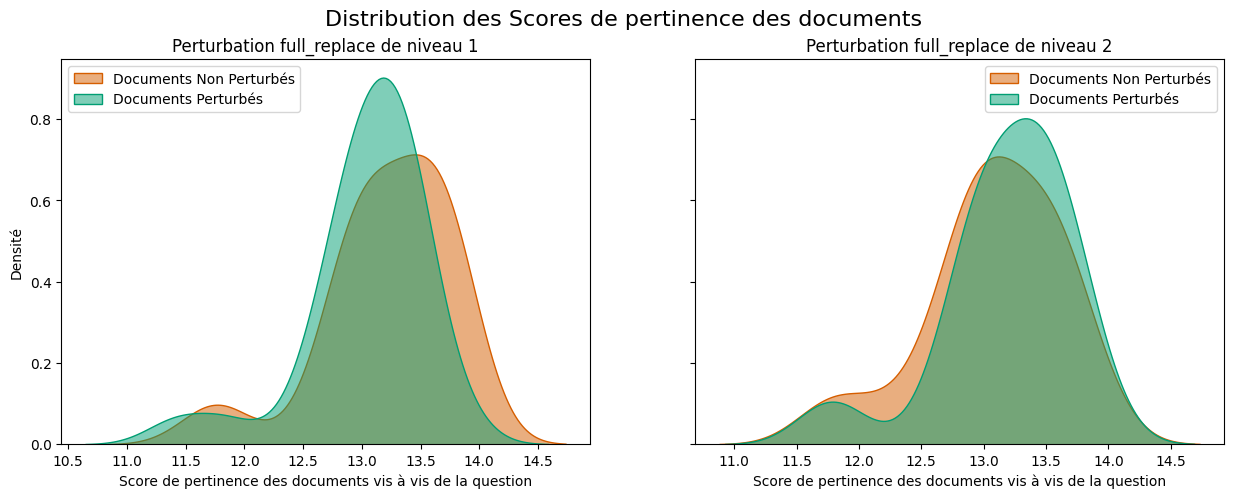
\includegraphics[width=0.8\linewidth]{images/PerturbationScoreExemple_FullReplace.png}
            \caption{Distribution des scores de pertinence pour les exemples de perturbation de type \fullreplace de niveau 1 et 2}
            \label{fig:pertFRNiv1-2}
        \end{figure}

        La Figure~\ref{fig:pertFRNiv1-2} représente les distributions des scores de pertinence pour deux perturbations de type \fullreplace. La première perturbation applique les 8 perturbation \replace de niveau 1 listées dans la table~\ref{tab:perturbations}. Par exemple, l'extrait 
        \begin{quote}
            Certaines limitations sont plus particulièrement liées aux caractéristiques du vecteur aérien et n’affectent donc pas toutes les catégories de drones de la même manière.
        \end{quote}
        devient
        \begin{quote}
            Certaines contraintes sont plus particulièrement liées aux caractéristiques du vecteur de vol et n’affectent donc pas toutes les catégories de vecteurs de la même manière.
        \end{quote}
        lorsqu'on applique cette perturbation. Les mots \textit{limitations}, \textit{aérien} et \textit{drones} ont tous les trois été remplacés. On peut considérer que cette perturbation est de niveau 1 car tous les remplacements effectués sont de niveau 1. La seconde perturbation regroupe les perturbation \replace de niveau 2 proposées dans la table~\ref{tab:perturbations}. C'est donc une perturbation de niveau 2. On constate que les perturbations de type \fullreplace impactent plus fortement la distribution des scores de pertinence que les perturbation \replace. 

        Lorsqu'on y regarde de plus près, une autre force des perturbations \fullreplace est leur capacité à couvrir plus facilement l'ensemble du dataset. Pour qu'un perturbation impacte le modèle, elle doit modifier les documents. Si une perturbation \replace modifie qu'une partie des documents alors elle aura moins d'impact sur le modèle Les documents non modifiés auront un score ramené à zéro (la division par zéro induit un NaN qui est interprété comme un zéro dans le calcul de la moyenne des scores de sensibilité pour tout le dataset). Les perturbations \fullreplace touchent plus de document car elles modifient l'union des documents modifiés par chacune d'entre elles. 
        
        

\section{Compléments pour l'estimation de la pertinence d'une perturbation}
%     \begin{verbatim}
% SI PAS DÉJÀ PRÉSENTÉ DANS PARTIE DE L'ÉTAT DE L'ART SUR MECHIR
% - On visualise des scores de similarité entre question et document
% - graphique d'exemple + texte d'accompagnement à la lecture
% - Un perturbation peut être considérée comme pertinente lorsqu'elle modifie significativement 
% (jugement humain) la distribution des cores pour l'échantillon du dataset étudié

% - on propose d'autres visualisations et confrontation de la distribution des scores entre perturbation :
%   - observation de la distribution des scores pour les documents pertinents et non-pertinents (sont-ils très séparés initialement?, Quel impact de la perturbation sur la distribution des documents pertinents/ non-pertinents?, La tendance est-elle systématique pour toutes les perturbations de même type? de même niveau?, pour un même mot cible?)
%   - observation de la distribution des scores d'un niveau de perturbation à l'autre pour un mot cible (quel comportement d'un niveau à l'autre? comportement commun à plusieurs mots?)

%     \end{verbatim}

     On propose de compléter l'estimation de la pertinence d'une perturbation proposée par \cite{parry_mechir_2025} à l'aide de deux autres visualisations qui mettent les perturbations en perspective vis a vis des données et entre elles.

     La première visualisation complémentaire est la visualisation des scores de pertinence en séparant les documents pertinents et non pertinents vis a vis de la question.  Cela permet de distinguer les effets de la perturbation sur chaque groupe de documents. On peut notamment d'identifier un impacts plus important des perturbations sur l'un des deux groupes (si le mot remplacé est plus présent dans les documents pertinents par exemple). Cette information pourra donner un éclairage différent sur la perturbation ou les nœuds identifiés comme sensibles au patching. 

     \begin{figure}
         \centering
         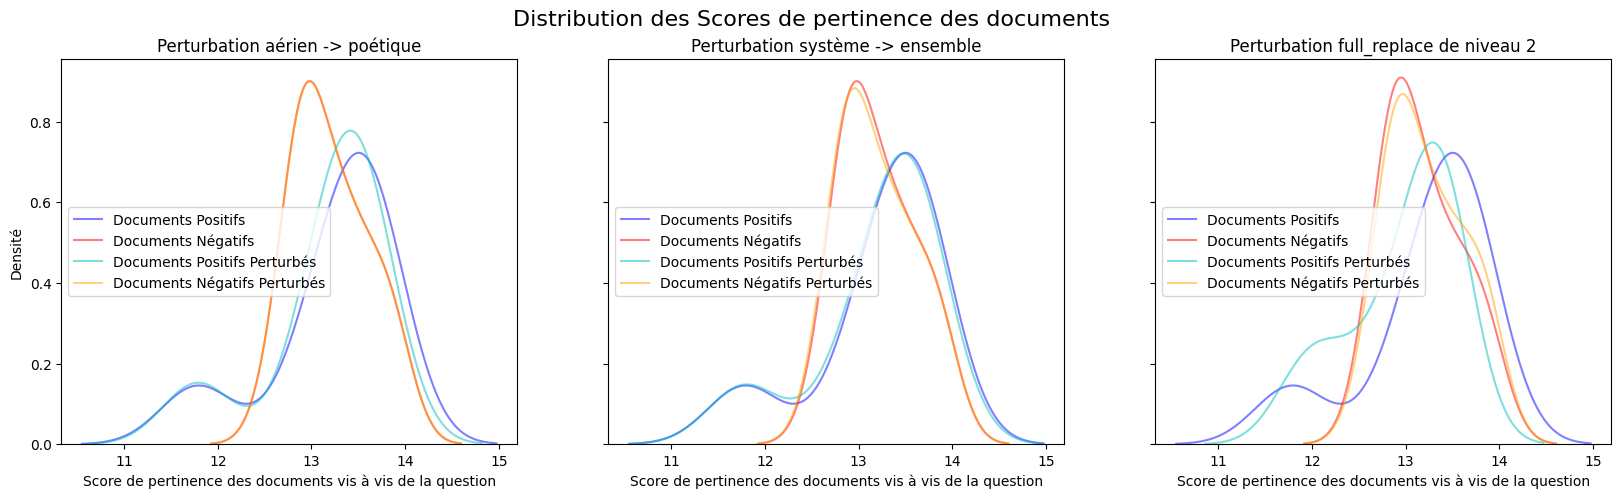
\includegraphics[width=\textwidth]{images/PerturbationScoreExemple_PosNeg.png}
         \caption{Distribution des scores de perturbation pour les documents positifs/négatifs (non-)perturbés pour trois perturbations}
         \label{fig:DistribScoresDocsPosNegSepares}
     \end{figure}

     Par exemple, dans la figure~\ref{fig:DistribScoresDocsPosNegSepares}, on s'intéresse au changement de distribution des scores pour les perturbations "remplacer \textit{aérien} par \textit{poétique}", "remplacer \textit{système} par \textit{ensemble}" et "remplacer tous les mots cible choisis par leur mot remplaçant de niveau 2" (voir la table~\ref{tab:perturbations}). On constate que les documents non pertinents vis-a-vis de la question ne changent pas de score de pertinence lorsqu'on applique la perturbation \textit{remplacer aérien par poétique} au dataset. Cela s'explique par le fait qu'aucun document non-pertinent ne contient le mot \textit{aérien}. On note que ce phénomène est assez répandu à cause de la méthode de construction du dataset. En effet, sélectionner des extraits issus de différents PDF portant sur différents sujets en lien avec la défense force les extraits à contenir un vocabulaire spécifique au sujet du PDF qui n'est pas nécessairement le même pour tous les PDFs utilisés. Dans notre cas, le seul mot remplacé ne subissant pas ce phénomène est \textit{système}. 


     La seconde visualisation complémentaire est la visualisation des distributions des scores à travers les différentes perturbations d'un même mot et à travers les différents niveaux de perturbation du mot. Cela permet de mettre en perspective les différentes perturbations et éventuellement de sélectionner la plus impactante au sein d'un même niveau. 

     \begin{figure}
         \centering
         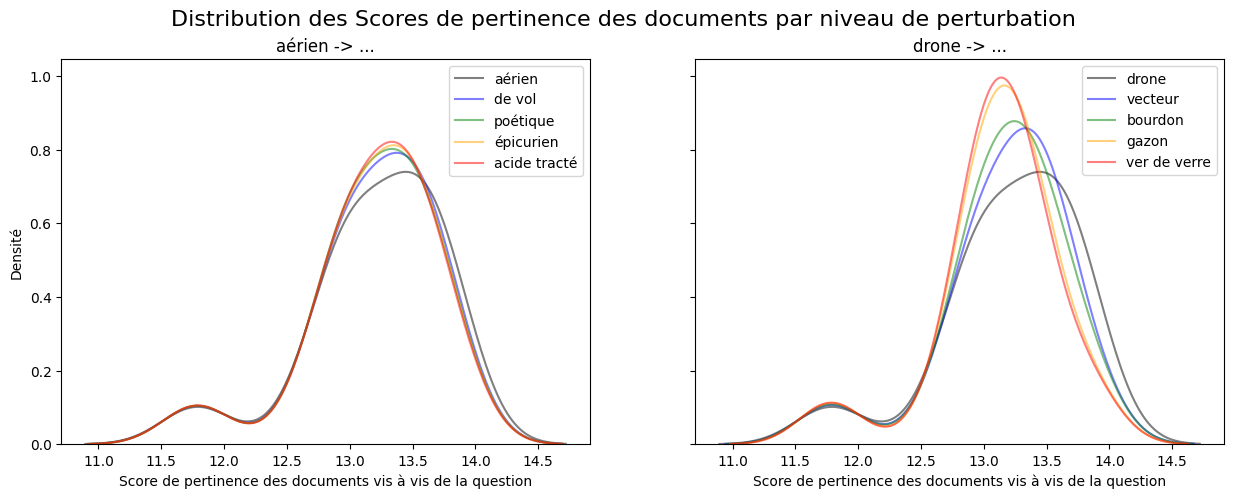
\includegraphics[width=\textwidth]{images/PerturbationScoreExemple_ParNiveaux.png}
         \caption{Distribution des scores de pertinence des documents pour les mots remplacés \textit{aérien} et \textit{drone}. La distribution des scores des documents non-perturbés et pour les 4 niveaux de perturbation appliqués sont regroupés dans le même graphique pour chaque mot}
         \label{fig:DistribScoresPerturbationParNiveaux}
     \end{figure}

     La visualisation des distributions des scores de pertinence des documents pour chaque perturbations appliquées à un même mot comme dans la figure~\ref{fig:DistribScoresPerturbationParNiveaux} permet de constater l'évolution de la distribution en fonction des niveaux de perturbation appliqués. On constate qu'elle n'est pas toujours très marquée. 

\section{Interprétation des résultats de l'Activation Patching}

    Un fois la ou les perturbations choisies, on peut appliquer l'activation patching à l'aide de l'outil MechIR. On propose dans cette partie des visualisations des résultats supplémentaires pour faciliter et/ou éclairer l'analyse et la cartographie du modèle.

    \subsection{Complément à la visualisation de la sensibilité du modèle à la perturbation}
        %\md{TODO : revoir le découpage de la partie une fois intégralement rédigée}
    
        \paragraph{Exploitation de l'écart-type} Pour rappel, \cite{parry_mechir_2025} propose de visualiser la moyenne des sensibilités du nœud à la perturbation appliquée sur chaque document. On propose de compléter le visualisation des moyennes par celle des écarts-types. Les moyennes de sensibilité peuvent être élevées (en valeur absolue)  à cause de rares documents qui modifiés impactent fortement le modèle. À contrario, certaines moyennes de sensibilité pourraient être proche de zéro à cause d'un effet de compensation entre les scores pour différents documents. Les écarts-types peuvent aider à distinguer les nœuds sensibles de façon homogène (à travers les documents) à une perturbation des nœuds subissant de façon plus importante du bruit.

        \begin{figure}
            \centering
            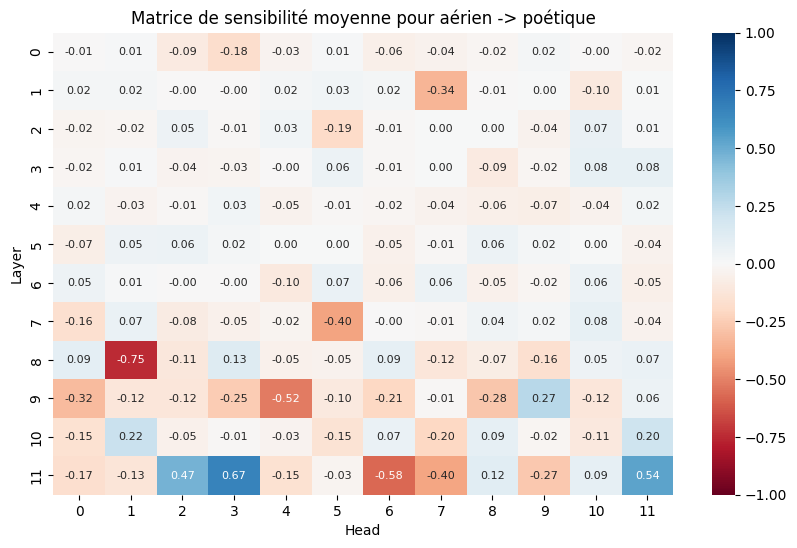
\includegraphics[width=0.48\textwidth]{images/MatriceSensibilite_old-mean_aerien-poetique.png}
            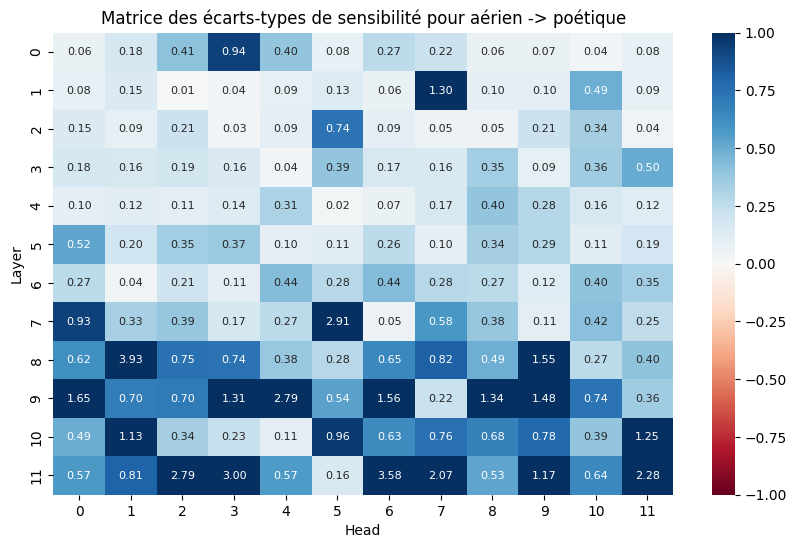
\includegraphics[width=0.48\textwidth]{images/MatriceSensibilite_old-std_aerien-poetique.png}
            \caption{Matrice de sensibilité moyenne et leurs écarts-types des nœuds pour la perturation "remplacer \textit{aérien} par \textit{poétique}"}
            \label{fig:MatriceSensibiliteOldAerienPoetique}
        \end{figure}

        La figure~\ref{fig:MatriceSensibiliteOldAerienPoetique} représente la sensibilité moyenne de chaque nœud de mE5 à la perturbation "remplacer \textit{aérien} par \textit{poétique}" à gauche et l'écart-type des sensibilités pour chaque documents pour les nœuds. On identifie bien les nœuds (8,1), (11,3), (9,4), (11,6) et (11,11) comme sensibles à l'aide de la matrice de sensibilités moyennes. Le nœud (11,2) est plus facilement identifiable à l'aide de la matrice des écarts-types de sensibilité. Cette matrice permet aussi de confirmer les premiers nœuds identifiés. 

        \paragraph{Adaptation de la visualisation des résultats de l'activation patching} D'une perturbation à l'autre, les nœuds ont des sensibilité moyennes très variables. Dans certains cas, les sensibilités ont un très faible écart-type (à travers la matrice) et dans d'autres, plusieurs nœuds saturent l'échelle de couleur proposée par MechIR. De la même façon, certains écarts-types explosent. De plus, par définition, un écart-type est positif. La moitié de l'échelle n'est alors par utilisée. \\
        Pour faciliter la visualisation, on propose de compléter la diversification des matrices de valeurs par une diversification des échelles de couleur. 
        Pour maintenir un accès aux valeurs exactes, on propose une échelle adaptative allant de -50 à 50 dans le cas de matrices de sensibilité ayant des nœuds avec un score de sensibilité moyen supérieur à 20. Pour les autres cas, on maintient l'échelle -1;1. On propose de conserver la même échelle de couleur mais de l'inverser afin que les valeurs positives soient en rouge et les valeurs négatives en bleu.
        
        En complément des matrices contenant les valeurs réelles, on propose une visualisation des valeurs ramenées dans l'intervalle -1;1 en maintenant zéro à sa valeur (division de toutes les valeurs par la sensibilité maximale en valeur absolue). On conserve la même échelle de couleur. Une telle visualisation permet de mettre en perspective les matrices d'une perturbation à l'autre : on peut comparer les nœuds ayant les sensibilités moyennes les plus élevées. D'autre part, cette approche permet d'identifier les nœuds significativement plus sensibles car ils seront plus foncés que les autres (valeurs proches de 1 en valeur absolue) et "se détachent" du reste des nœuds. Pour le cas des écarts-types, on propose les mêmes échelles mais en tronquant à 0 et avec la gamme de couleurs Noir-Violet-Orange-Jaune.

        \begin{figure}
            \centering
            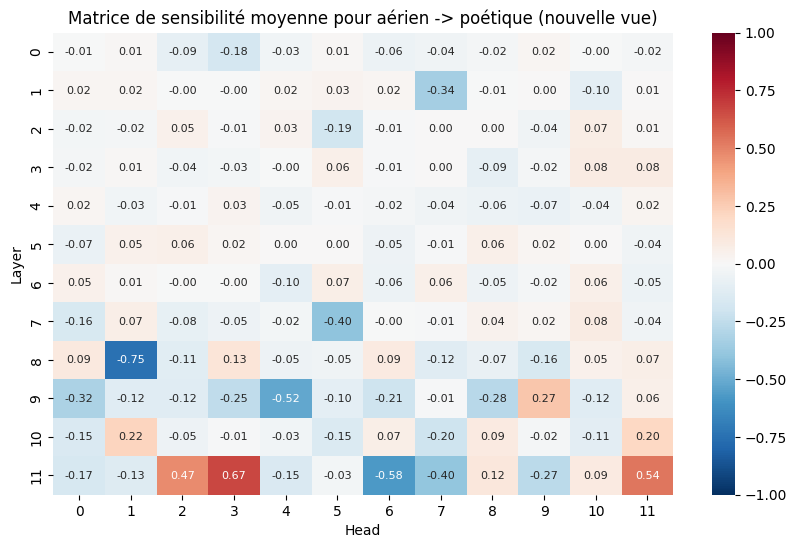
\includegraphics[width=0.48\textwidth]{images/MatriceSensibilite_new-mean_aerien-poetique.png}
            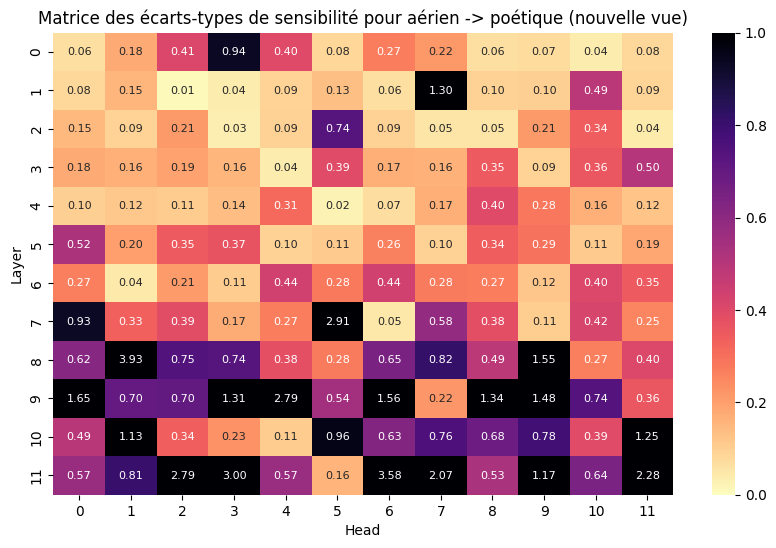
\includegraphics[width=0.48\textwidth]{images/MatriceSensibilite_new-std_aerien-poetique.png}
            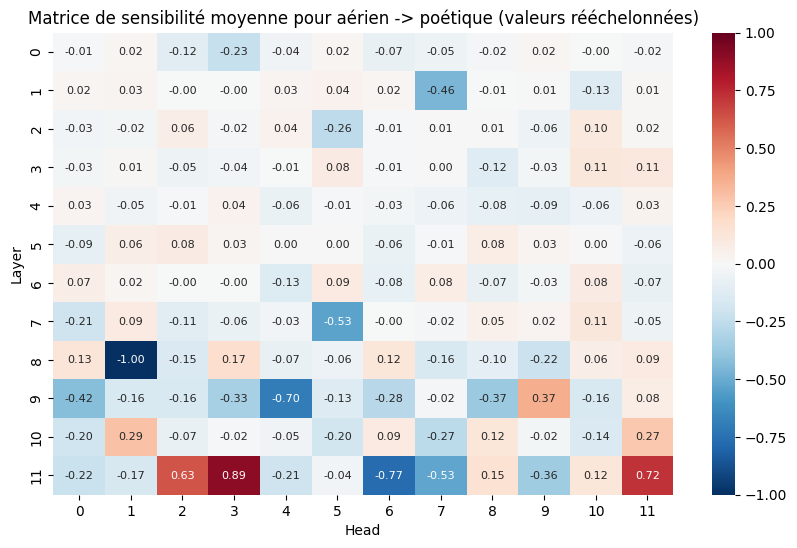
\includegraphics[width=0.48\textwidth]{images/MatriceSensibilite_resc-mean_aerien-poetique.png}
            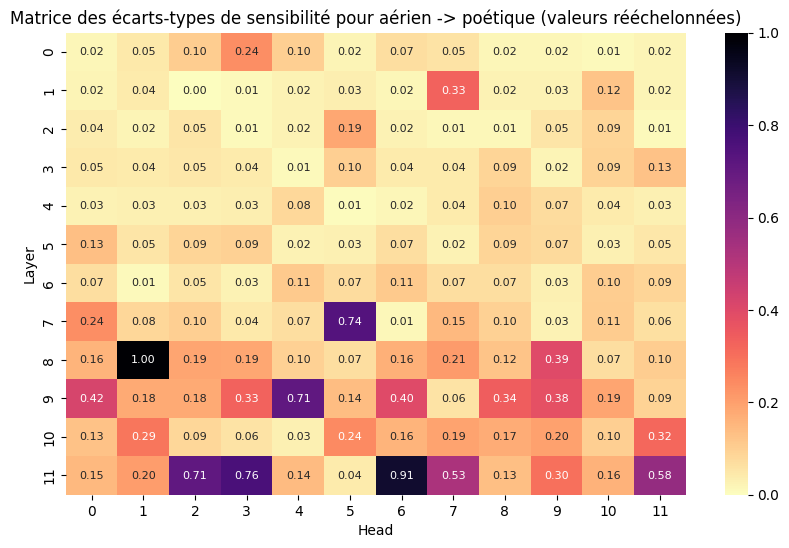
\includegraphics[width=0.48\textwidth]{images/MatriceSensibilite_resc-std_aerien-poetique.png}
            \caption{Matrice de sensibilité moyenne et leurs écarts-types des nœuds pour la perturbation "remplacer \textit{aérien} par \textit{poétique}" avec la nouvelle visualisation (en haut) et avec le rééchelonnage (en bas)}
            \label{fig:MatriceSensibiliteNewAerienPoetique}
        \end{figure}

        La figure~\ref{fig:MatriceSensibiliteNewAerienPoetique} affiche les mêmes données que la figure~\ref{fig:MatriceSensibiliteOldAerienPoetique} en appliquant la nouvelle échelle de couleurs et les nouvelles bornes et en appliquant le rééchelonnage. Le rééchelonnage permet de faciliter l'identification des nœuds en exploitant l'intégralité de l'échelle de couleur. On repère notamment le nœud (7,5) pour lequel l'identification comme nœud sensible était plus incertaine avec la visualisation précédente. 
        
    
    %\md{à placer : confronter les matrices d'une perturbation à l'autre}
%         \begin{verbatim}

% - étant donné la construction de ces valeurs, on s'intéresse aussi aux écarts-types
% - pour faciliter la visualisation et la comparaison en cas de sensibilité variable 
% d'une perturbation à l'autre on propose de rescaler les poids des matrices
%         \end{verbatim}

    \subsection{Critère d'identification des nœuds sensibles}
%         \begin{verbatim}
% - L'identification des nœuds sensibles doit reposer sur un critère commun. On propose
% un critère de sensibilité ...
%         \end{verbatim}

        L'identification des nœuds sensibles et un étape importante pour la cartographie d'un modèle. Distinguer les nœuds sensibles des nœuds qui ne le sont pas doit reposer sur un critère commun à toutes le perturbations. De plus, un critère automatisable voire quantitatif permet une détection de ces nœuds plus facile et rapide. On propose un critère de sensibilité qui prend en compte les différentes données visualisées précédemment. On considère un nœud comme sensible si le score de sensibilité moyenne est supérieur à 0.1 en valeur absolue et le score de sensibilité moyenne normalisé est supérieur à 0.5 en valeur absolue. Ainsi, seul les nœuds impactés significativement sont considérés dans le cas où ils "se détachent" du reste des nœuds. En complément du double critère sur la sensibilité moyenne, on ajoute second un double critère sur l'écart-type des sensibilité du nœud. Un nœud peut être sensible si son écart-type est supérieur à 0.1 et que son écart-type normalisé est supérieur à 0.5. Ainsi, les nœuds ayant une moyenne proche de zéro à cause d'un effet d'équilibrage entre les documents est tout de même considéré comme un nœud sensible à la perturbation appliquée aux documents. Pour récapituler, un nœud est considéré comme sensible si il vérifie la condition suivante:

        $$((\mid mean \mid > 0.1) \wedge (\mid resc\_mean \mid > 0.5) ) \vee ( (std > 0.1) \wedge (resc\_std > 0.5))$$

        Il faut tout de même noter que le choix des bornes 0.5 et 0.1 sont intéressantes pour le dataset utilisé au cours du stage mais pourraient être à ajuster lors de l'utilisation d'autres datasets. 

    \subsection{Matrice des nœuds sensibles}
%         \begin{verbatim}
% - Pour faciliter le besoin de mise en perspective des matrice de sensibilité d'un perturbation à l'autres ...
% - Visualisation des nœuds sensibles **commun à plusieurs perturbation** (matrice des nœuds sensibles)
%     -> croiser les différentes caractéristiques (mot remplacé, type, niveau)
%     -> critique des nœuds sensibles de la dernière couche
%         \end{verbatim}

        Pour considérer qu'un nœud traite une notion de langage ou de raisonnement (identifie le vocabulaire de spécialité par exemple), il doit être sensible à plusieurs des perturbations visant cette compétence. On peut aussi s'intéresser à la persistance de cette sensibilité à travers différents datasets similaires pour une même perturbation ou à travers différentes perturbations similaires pour un même dataset. Pour faciliter cette analyse de la persistance de la sensibilité d'un nœud, on propose de visualiser la matrice des nœuds sensibles. Pour chaque nœud, repéré par ses coordonnées, elle indique le nombre de perturbations pour lesquelles le nœud est considéré comme sensible au regard du critère présenté dans la sous-section précédente. 

        \begin{figure}
            \centering
            \begin{subfigure}[b]{0.5\textwidth}
                \centering
                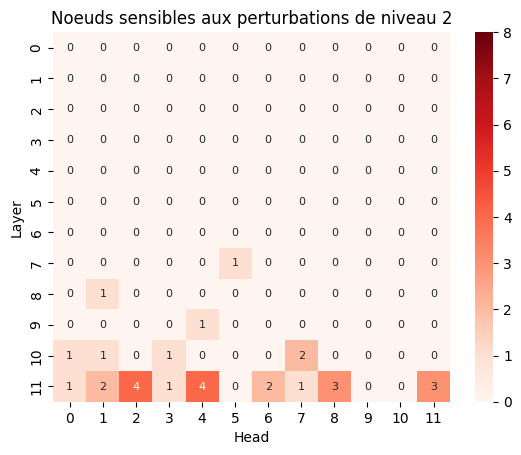
\includegraphics[width=\textwidth]{images/NoeudsSensiblesNiv2.png}
                \caption{Nombre de perturbations de niveau 2 impactant les nœuds du modèle}
            \end{subfigure}%
            ~ 
            \begin{subfigure}[b]{0.5\textwidth}
                \centering
                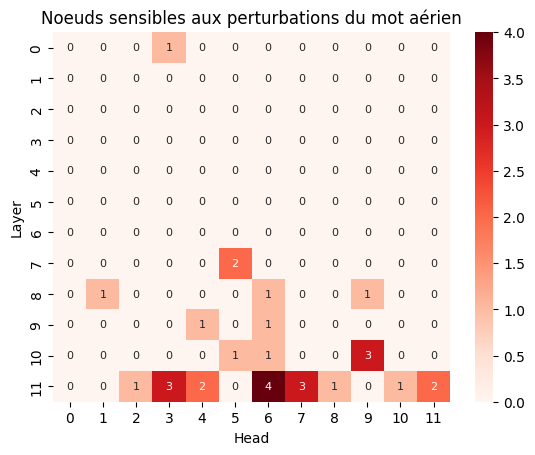
\includegraphics[width=\textwidth]{images/NoeudsSensiblesAerien.png}
                \caption{Nombre de perturbations appliquées à \textit{aérien} impactant les nœuds du modèle}
            \end{subfigure}
            \caption{Matrices de nœuds sensibles}
            \label{fig:MatNoeudsSensibles}
        \end{figure}

        La figure~\ref{fig:MatNoeudsSensibles} illustre deux usages des matrices de nœuds sensibles. La première compte le nombre de fois qu'un nœud est sensible aux perturbations décrites par la troisième colonne de  la table~\ref{tab:perturbations}. On constate qu'aucune tendance ne se dégage : les nœuds les plus sensibles ne le sont que pour la moitié des perturbations. La seconde matrice s'intéresse à la sensibilité des nœuds pour une ensemble de perturbations portant sur le même mot. On s'intéresse aux quatre perturbations de quatre niveau différents appliquées au mot \textit{aérien}. Le nœud (11,6) est sensible aux quatre perturbations et les nœuds (11,3), (11,7) et (10,9) sont sensible à trois des quatre perturbations étudiées. 